\documentclass{article}
\usepackage{amsmath}
\usepackage{amssymb}
\usepackage{graphicx}
\usepackage{tikz}
\usepackage{pgfplots}
\usepackage{listings}
\usepackage{xcolor}
\usepackage{hyperref}
\usepackage{booktabs}
\usepackage{multirow}
\usetikzlibrary{shapes,arrows,positioning,calc}

\definecolor{codegreen}{rgb}{0,0.6,0}
\definecolor{codegray}{rgb}{0.5,0.5,0.5}
\definecolor{codepurple}{rgb}{0.58,0,0.82}
\definecolor{backcolour}{rgb}{0.95,0.95,0.92}

\lstdefinestyle{mystyle}{
    backgroundcolor=\color{backcolour},
    commentstyle=\color{codegreen},
    keywordstyle=\color{magenta},
    numberstyle=\tiny\color{codegray},
    stringstyle=\color{codepurple},
    basicstyle=\ttfamily\footnotesize,
    breakatwhitespace=false,
    breaklines=true,
    captionpos=b,
    keepspaces=true,
    numbers=left,
    numbersep=5pt,
    showspaces=false,
    showstringspaces=false,
    showtabs=false,
    tabsize=2
}

\lstset{style=mystyle}

\title{Simulation of Cellular Reprogramming and Rejuvenation: A Computational Model}
\author{Witold Warchoł}
\date{\today}

\begin{document}

\maketitle

\section{Abstract}
This paper presents a computational model of cellular reprogramming and rejuvenation, simulating key biological processes such as DNA repair, telomerase activation, epigenetic reset, and mitochondrial replacement. The model integrates probabilistic outcomes and system-level coordination to explore the feasibility and dynamics of cellular rejuvenation.

\section{Introduction}
Aging is characterized by the accumulation of cellular damage, including DNA mutations, telomere shortening, protein aggregation, and mitochondrial dysfunction. Cellular reprogramming offers a promising approach to reverse these hallmarks of aging. This paper describes a simulation framework that models these processes and their potential reversal through a series of coordinated phases.

\section{Model Overview}
The simulation models a hierarchical system of cells, tissues, and organs, each with specific attributes and processes. The model progresses through a sequence of reprogramming phases, each targeting a distinct hallmark of aging.

\subsection{Reprogramming Phases}
The simulation is divided into the following phases:
\begin{itemize}
    \item Initialization
    \item Homeostasis Establishment
    \item DNA Repair Activation
    \item Telomerase Activation
    \item Epigenetic Reset
    \item Tissue Rejuvenation
    \item Protein Aggregate Removal
    \item Mitochondrial Replacement
    \item Senescent Cell Removal
    \item Coordination Verification
\end{itemize}

\subsection{System Components}
The model consists of the following components:
\begin{itemize}
    \item \textbf{Cells}: Represented with attributes such as telomere length, DNA damage, protein aggregates, and mitochondrial health.
    \item \textbf{Tissues}: Composed of cells, with metrics for homeostasis and metabolic balance.
    \item \textbf{Organs}: Composed of tissues, with coordination and health metrics.
\end{itemize}

\section{Mathematical Framework}
Each phase of the simulation is governed by probabilistic and deterministic rules, reflecting the biological variability and complexity of cellular processes.

\subsection{Probability Calculations}
The success of each phase is determined by a probability function, \( P_{\text{phase}} \), which depends on system metrics such as average health, DNA integrity, and metabolic efficiency. For example, the probability of successful DNA repair activation is given by:

\[
P_{\text{DNA Repair}} = \left( \frac{\text{repairable\_cells}}{\text{total\_cells}} \right) \times \left(1 - \frac{\text{damage\_burden}}{2}\right) \times 0.70
\]

\subsection{Phase-Specific Metrics}
Each phase calculates specific metrics to determine success:
\begin{itemize}
    \item \textbf{DNA Repair Activation}: Assesses DNA integrity and repair efficiency.
    \item \textbf{Telomerase Activation}: Measures telomere length improvement.
    \item \textbf{Epigenetic Reset}: Tracks the number of reprogrammed cells.
    \item \textbf{Mitochondrial Replacement}: Evaluates the reduction in defective mitochondria.
\end{itemize}

\section{Biological Visualizations}

\subsection{Cellular Reprogramming Process}
\begin{figure}[h]
\centering
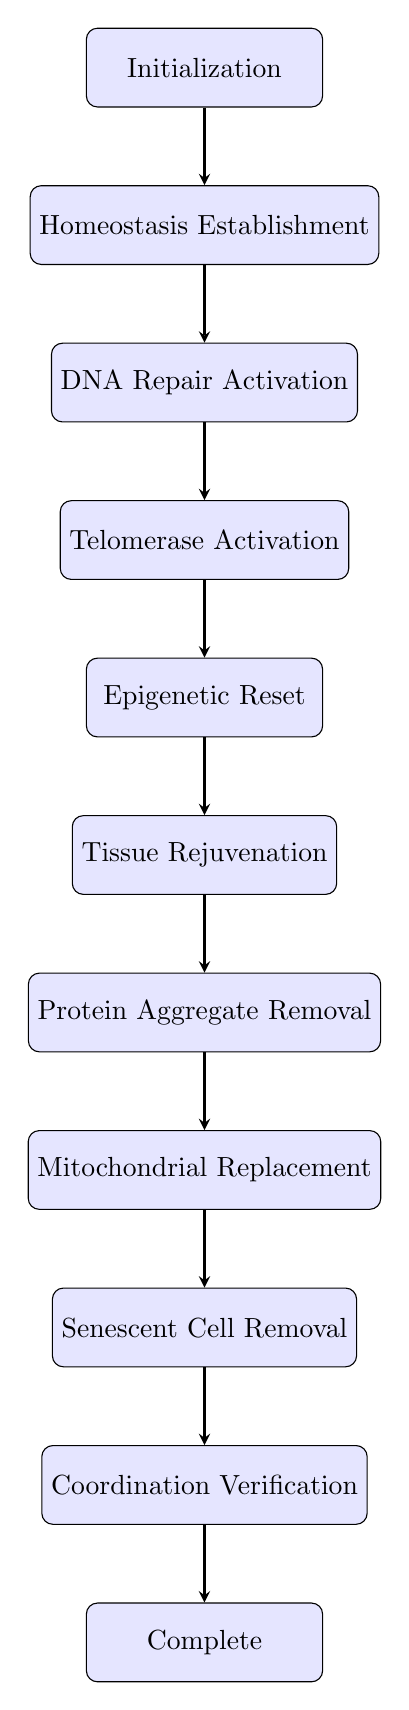
\begin{tikzpicture}[node distance=2cm, auto]
    \tikzstyle{phase} = [rectangle, rounded corners, minimum width=3cm, minimum height=1cm, text centered, draw=black, fill=blue!10]
    \tikzstyle{arrow} = [thick,->,>=stealth]

    \node (init) [phase] {Initialization};
    \node (homeostasis) [phase, below of=init] {Homeostasis Establishment};
    \node (dna) [phase, below of=homeostasis] {DNA Repair Activation};
    \node (telomerase) [phase, below of=dna] {Telomerase Activation};
    \node (epigenetic) [phase, below of=telomerase] {Epigenetic Reset};
    \node (rejuvenation) [phase, below of=epigenetic] {Tissue Rejuvenation};
    \node (protein) [phase, below of=rejuvenation] {Protein Aggregate Removal};
    \node (mitochondrial) [phase, below of=protein] {Mitochondrial Replacement};
    \node (senescent) [phase, below of=mitochondrial] {Senescent Cell Removal};
    \node (coordination) [phase, below of=senescent] {Coordination Verification};
    \node (complete) [phase, below of=coordination] {Complete};

    \draw [arrow] (init) -- (homeostasis);
    \draw [arrow] (homeostasis) -- (dna);
    \draw [arrow] (dna) -- (telomerase);
    \draw [arrow] (telomerase) -- (epigenetic);
    \draw [arrow] (epigenetic) -- (rejuvenation);
    \draw [arrow] (rejuvenation) -- (protein);
    \draw [arrow] (protein) -- (mitochondrial);
    \draw [arrow] (mitochondrial) -- (senescent);
    \draw [arrow] (senescent) -- (coordination);
    \draw [arrow] (coordination) -- (complete);
\end{tikzpicture}
\caption{Flowchart of the cellular reprogramming phases.}
\label{fig:reprogramming_phases}
\end{figure}

\subsection{Mitochondrial Health Dynamics}
\begin{figure}[h]
\centering
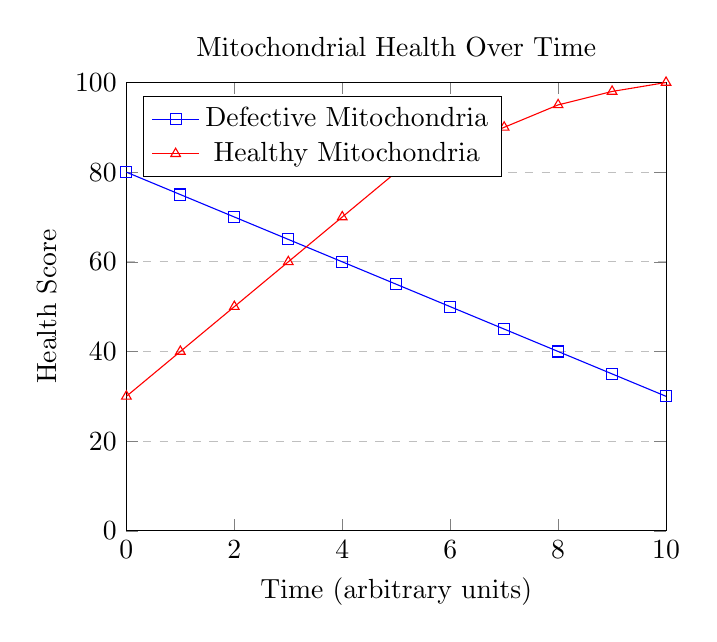
\begin{tikzpicture}
    \begin{axis}[
        title={Mitochondrial Health Over Time},
        xlabel={Time (arbitrary units)},
        ylabel={Health Score},
        xmin=0, xmax=10,
        ymin=0, ymax=100,
        xtick={0,2,4,6,8,10},
        ytick={0,20,40,60,80,100},
        legend pos=north west,
        ymajorgrids=true,
        grid style=dashed,
    ]
    \addplot[
        color=blue,
        mark=square,
        ]
        coordinates {
        (0,80)(1,75)(2,70)(3,65)(4,60)(5,55)(6,50)(7,45)(8,40)(9,35)(10,30)
        };
    \addplot[
        color=red,
        mark=triangle,
        ]
        coordinates {
        (0,30)(1,40)(2,50)(3,60)(4,70)(5,80)(6,85)(7,90)(8,95)(9,98)(10,100)
        };
    \legend{Defective Mitochondria, Healthy Mitochondria}
    \end{axis}
\end{tikzpicture}
\caption{Dynamics of mitochondrial health during the reprogramming process.}
\label{fig:mitochondrial_health}
\end{figure}

\section{Simulation Workflow}
The simulation proceeds as follows:
\begin{enumerate}
    \item Initialize the system with a defined number of cells, tissues, and organs.
    \item Execute each phase in sequence, calculating success probabilities and updating system metrics.
    \item Adjust parameters between attempts to improve success rates.
    \item Repeat the sequence for a maximum number of attempts or until success is achieved.
\end{enumerate}

\section{Results and Discussion}
The simulation provides detailed statistics for each phase, including success rates, average improvements, and system-level metrics. These results can be used to explore the dynamics of cellular reprogramming and identify critical factors influencing success.

\subsection{Example Output}
\begin{table}[h]
\centering
\caption{Example Phase Statistics}
\begin{tabular}{lc}
\toprule
\textbf{Phase} & \textbf{Success Rate} \\
\midrule
Initialization & 0.85 \\
DNA Repair Activation & 0.78 \\
Telomerase Activation & 0.82 \\
Epigenetic Reset & 0.75 \\
\bottomrule
\end{tabular}
\end{table}

\subsection{Mathematical Formulas}
The success probability for the \textbf{DNA Repair Activation} phase is calculated as:

\[
P_{\text{DNA Repair}} = \left( \frac{N_{\text{repairable}}}{N_{\text{total}}} \right) \times \left(1 - \frac{D}{2}\right) \times 0.70
\]

where:
\begin{itemize}
    \item \(N_{\text{repairable}}\) is the number of repairable cells.
    \item \(N_{\text{total}}\) is the total number of cells.
    \item \(D\) is the damage burden, calculated as \(D = 1 - \frac{\text{avg\_integrity}}{100}\).
\end{itemize}

\section{Conclusion}
This simulation framework provides a powerful tool for exploring the dynamics of cellular reprogramming and rejuvenation. By integrating probabilistic outcomes and system-level coordination, the model offers insights into the feasibility and optimization of cellular rejuvenation strategies.

\section*{Acknowledgments}
This work was inspired by recent advances in cellular reprogramming and computational biology.

\end{document}
